%!TeX root=20_Hauptteil.tex

%\chapter{Implementierung der Positionierung}
%
%\subsection{Kommunikation PX4}
%
%\subsection{Flugsteuerung}
%
%\section{Bildaufnahme}
%
%\subsection{Kamerakalibrierung}
%
%\section{Entzerrung}
%
%\section{Bildverarbeitung}
%
%\section{Positionsbestimmung}
%
%\subsection{extrinsische Kamerakalibrierung}

%!TeX root=20_Hauptteil.tex
\chapter{Implementierung der Positionierung}
\label{cap:lokalisierung}
Dieses Kapitel beschreibt die im Flug ablaufende Positionsbestimmung des Fluggeräts.
Im Gegensatz zur Kartierung (Kapitel~\ref{cap:kartierung}) läuft die Verarbeitung hier zur Laufzeit auf dem Companion-Computer.
Die Kette folgt dem in Abschnitt~\ref{sec:softwarearchitektur} dargestellten Datenfluss: Bildaufnahme, Entzerrung, Bildverarbeitung, Positionsbestimmung, 
Kommunikation mit der Flugsteuerung und schließlich die Flugsteuerung selbst.
Die ersten drei Schritte entsprechen methodisch denen der Kartierung, werden aber mit höherer Bildrate und auf der GPU des Jetson ausgeführt.
In nachfolgenden Abschnitt wird auf die konkrete Softwarearchitektur zur Positionierung eingegangen. 

\section{Softwarearchitektur der Positionierung}
\label{sec:softwarearchitektur_positionierung}
Die Positionierung ist auf zwei Ausführungsumgebungen aufgeteilt: den Host des Companion-Computers und einen Container.
Diese Trennung ergibt sich aus der Verwendung von Isaac~ROS für die hardwarebeschleunigten Schritte.
Isaac~ROS ist eine von NVIDIA bereitgestellte Sammlung von ROS2-Paketen, die für die Ausführung auf den \glspl{gpu} der Jetson-Plattform optimiert sind.
Die Pakete werden in einem vorkonfigurierten Container ausgeführt, der die benötigten Bibliotheken und Treiber bereitstellt.
Innerhalb dieses Containers werden die Entzerrung und die Markererkennung auf der \gls{gpu} ausgeführt, was gegenüber 
einer CPU-basierten Verarbeitung eine höhere Bildrate ermöglicht.
Die übrigen Schritte laufen direkt auf dem Host des Jetson.
Dort erfolgen die Bildaufnahme über gscam, die Positionsbestimmung aus den Markerdetektionen sowie die Kommunikation mit der Flugsteuerung.
Container und Host kommunizieren über ROS2-Topics.
Der Datenfluss zwischen den Knoten ist in Abbildung~\ref{fig:architektur_positionierung} dargestellt.
Die Bildaufnahme stellt das Kamerabild auf \topic{/camera_1/image_raw} mit den zugehörigen Parametern auf \topic{/camera_1/camera_info} bereit.
Im Container entzerrt der Knoten \texttt{RectifyNode} das Bild und gibt es als \topic{/camera_1/image_rect} aus.
Der Knoten \texttt{AprilTagNode} detektiert darauf die Marker und veröffentlicht die Detektionen auf \topic{/camera_1/tag_detections}.
Auf dem Host bestimmt der Knoten \texttt{vision\_pose\_uxrce\_node} aus diesen Detektionen die Pose des Fluggeräts und übergibt sie über \topic{/fmu/in/vehicle_visual_odometry} an die Flugsteuerung.

% TODO: Abbildung -- Knoten und Topics, getrennt nach Host und Container.
\begin{figure}[htbp]
    \centering
    % 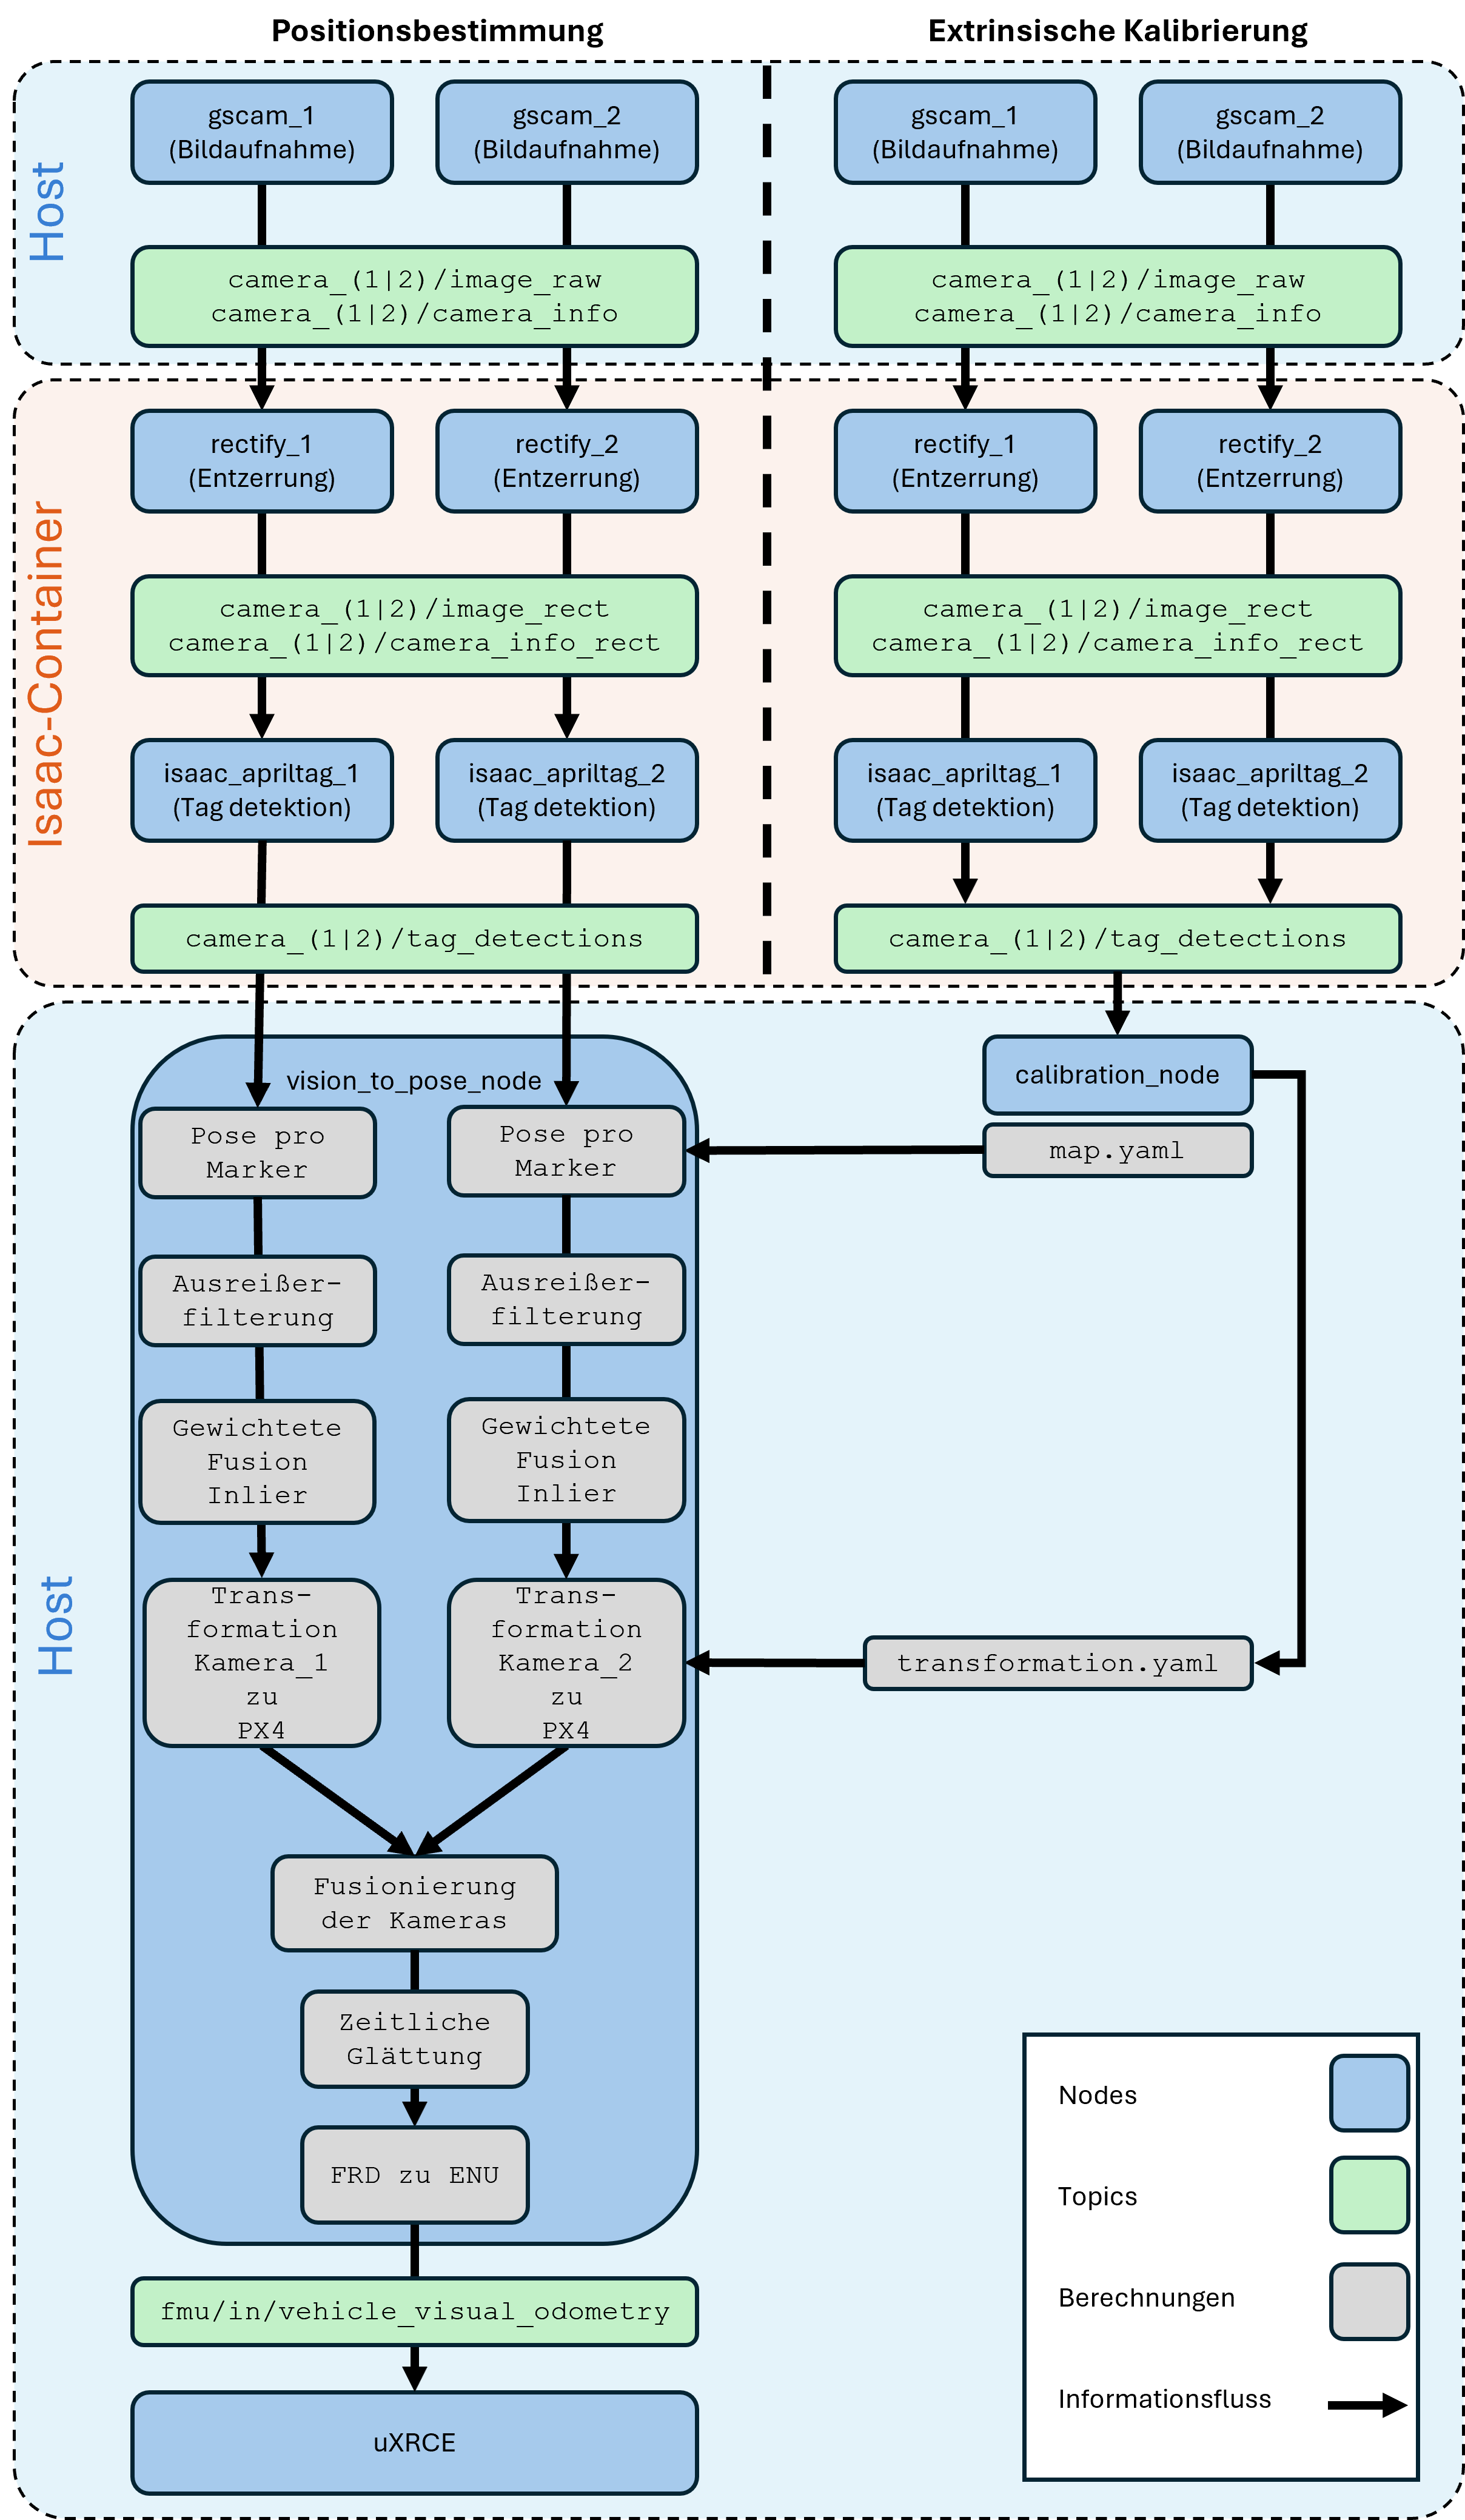
\includegraphics[width=\textwidth]{Bilder/Architektur_Positionierung.png}
    \caption{Knoten und Topics der Positionierung, aufgeteilt nach Host und Container}
    \label{fig:architektur_positionierung}
\end{figure}
\FloatBarrier





\section{Bildaufnahme Positionierung}
\label{sec:pos_bildaufnahme}
Die Bildaufnahme erfolgt wie bei der Kartierung (Abschnitt~\ref{sec:kartierung_bildaufnahme}) über einen gscam-Knoten.
Auch hier wird wie bei der Implementierung der Kartierung exemplarisch die Logitech~C922 verwendet.
Wie in Abschnitt~\ref{Kamera_Kalibrierung} beschrieben, muss die Kalibrierung für jede Kamera und für die hier verwendete 
Auflösung von $1280 \times 720$ Pixeln durchgeführt werden.


Listing~\ref{lst:gscam_node_pos} zeigt die geänderte Konfiguration.


\begin{lstlisting}[language=Python, caption={Parameter des gscam-Knotens zur Bildaufnahme im Flug}, label={lst:gscam_node_pos}]
'gscam_config': (
    'v4l2src device=/dev/video0 do-timestamp=true ! '
    'image/jpeg,width=1280,height=720,framerate=60/1 ! '
    'queue leaky=downstream max-size-buffers=1 ! '
    'nvv4l2decoder mjpeg=1 ! '
    'queue leaky=downstream max-size-buffers=1 ! '
    'nvvidconv ! '
    'video/x-raw,format=BGRx ! '
    'videoconvert ! '
    'video/x-raw,format=RGB,framerate=60/1'
),
'camera_name': 'camera_1',
'frame_id': 'camera_1_optical_frame',
'camera_info_url': camera_info_url,
'use_gst_timestamps': True,
'sync_sink': False,
'preroll': False,
'image_encoding': 'rgb8',
'use_sensor_data_qos': False,
\end{lstlisting}

Die beiden wesentlichen Unterschiede betreffen die Bildrate und die Dekodierung.
Die Kamera wird hier mit einer Auflösung von $1280 \times 720$ Pixeln bei $60$ \gls{fps} betrieben.
Die deutlich höhere Bildrate ist notwendig, da die Positionsbestimmung im Flug fortlaufend erfolgt und eine geringe Latenz erfordert.
Die Auflösung von $1280 \times 720$ Pixeln wurde gewählt, da die Logitech~C922 nur bei dieser Auflösung $60$ \gls{fps} liefert.
Möglich wird die hohe Bildrate durch die hardwarebeschleunigte Dekodierung des MJPEG-Streams über \texttt{nvv4l2decoder} und \texttt{nvvidconv} 
auf der \gls{gpu} des Jetson.
Ohne die hardwarebeschleunigte Dekodierung sinkt die Bildrate über die Zeit, da die CPU mit der Dekodierung 
nicht hinterherkommt und ein Puffer in der Pipeline volläuft.


\subsection{Kamerakalibrierung Positionierung}
\label{sec:pos_kalibrierung}
Schreibe mir den Abschnitt zur Kalibrierung.
sag dass für die neue Auflösung neue Parameter nach dem referenzierten Abschnitt ermittelt werden müssen. 



\subsection{Kamerakalibrierung Positionierung}
\label{sec:pos_kalibrierung}
Die intrinsische Kalibrierung der Flugkamera folgt demselben Lochkameramodell und Verzeichnungsmodell wie in Abschnitt~\ref{sec:kalibrieren_kamera} beschrieben.
Die Kalibrierung wird für das im Flug verwendete $1280 \times 720$-Profil separat durchgeführt, da Brennweite und Hauptpunkt von der Auflösung abhängen.
% TODO: Kalibrierwerte der Flugkamera (1280x720) ergaenzen.
Das Ergebnis wird als \texttt{camera\_info} bereitgestellt und in der nachfolgenden Entzerrung verwendet.


\section{ab hier ist vorsicht geboten}



\section{Entzerrung}
\label{sec:pos_entzerrung}
Die Entzerrung erfolgt im Flug über den Knoten \texttt{RectifyNode} aus dem Paket isaac\_ros\_image\_proc.
Dieser Knoten läuft GPU-beschleunigt innerhalb eines Composable-Node-Containers und entfernt die Verzeichnung anhand der Kalibrierparameter.
Das entzerrte Bild wird als \texttt{/camera\_1/image\_rect} mit den zugehörigen Parametern \texttt{/camera\_1/camera\_info\_rect} ausgegeben.
Wie in der Kartierung gilt: Nach der Entzerrung sind die Verzeichnungskoeffizienten null, und es werden die Parameter der Projektionsmatrix verwendet.

\section{Bildverarbeitung}
\label{sec:pos_bildverarbeitung}
Die Markererkennung übernimmt der Knoten \texttt{AprilTagNode} aus dem Paket isaac\_ros\_apriltag.
Er detektiert im entzerrten Bild Marker der Familie \texttt{tag36h11} mit einer konfigurierten Größe von $0{,}167\,\text{m}$ und maximal $40$ Markern pro Bild.
Die Detektion läuft GPU-beschleunigt und ist über das NITROS-Framework speichereffizient an die Entzerrung gekoppelt.
Für jeden erkannten Marker liefert der Knoten dessen Identifikationsnummer sowie die relative Pose zwischen Kamera und Marker als Topic \texttt{/camera\_1/tag\_detections}.
Diese Detektionen bilden den Eingang der Positionsbestimmung.

\section{Positionsbestimmung}
\label{sec:pos_positionsbestimmung}
Die Positionsbestimmung übernimmt der Knoten \texttt{vision\_pose\_uxrce\_node}.
Er berechnet aus den Markerdetektionen die Pose des Fluggeräts in der Karte und übergibt sie an die Kommunikation.
Der Ablauf gliedert sich in vier Schritte: die Posenberechnung je Marker, die Ausreißerfilterung, die gewichtete Fusion und die Umrechnung auf den Drohnenmittelpunkt.

\subsection{Posenberechnung je Marker}
Jede Detektion liefert die Transformation $\mathbf{T}_{\text{camera}}^{\text{tag}}$ zwischen Kamera und Marker.
Da die Lage jedes Markers in der Karte aus der Kartierung bekannt ist ($\mathbf{T}_{\text{map}}^{\text{tag}}$), lässt sich daraus die Kamerapose in der Karte berechnen:
\begin{equation}
    \mathbf{T}_{\text{map}}^{\text{camera}}
    = \mathbf{T}_{\text{map}}^{\text{tag}} \cdot \left(\mathbf{T}_{\text{camera}}^{\text{tag}}\right)^{-1}.
    \label{eq:tmap_camera}
\end{equation}
Jeder sichtbare Marker erzeugt somit eine eigene Hypothese für die Kamerapose.
Jeder Hypothese wird ein Gewicht zugewiesen, das mit dem Quadrat der Markerdistanz $d$ abnimmt:
\begin{equation}
    w = \frac{1}{d^{2}}.
    \label{eq:weight}
\end{equation}
Nahe Marker werden dadurch stärker gewichtet, da ihre Posenschätzung genauer ist.

\subsection{Ausreißerfilterung}
Bei mehreren sichtbaren Markern müssen die Hypothesen aus Gleichung~\eqref{eq:tmap_camera} übereinstimmen.
Fehldetektionen oder mehrdeutige Markerposen erzeugen jedoch abweichende Hypothesen.
Diese werden über ein RANSAC-Verfahren entfernt, das das größte Set konsistenter Hypothesen (Inlier) sucht.
Da das Rauschen der Posenschätzung mit der Distanz quadratisch zunimmt, wird die Inlier-Schwelle $\tau$ distanzabhängig skaliert:
\begin{equation}
    \tau = \tau_{\text{base}} \cdot \left(\frac{d_{\text{mean}}}{d_{\text{ref}}}\right)^{2},
    \label{eq:ransac_schwelle}
\end{equation}
mit der Basisschwelle $\tau_{\text{base}} = 0{,}015\,\text{m}$ bei der Referenzdistanz $d_{\text{ref}} = 0{,}30\,\text{m}$.
Ein Konsens gilt erst ab einem Inlier-Anteil von $70\,\%$ als zuverlässig.
Bei wenigen Markern wird das Set vollständig durchsucht, was die Filterung über aufeinanderfolgende Bilder deterministisch macht.

\subsection{Gewichtete Fusion}
Die verbleibenden Inlier-Hypothesen werden zu einer Kamerapose zusammengefasst.
Die Position ergibt sich als gewichtetes Mittel über alle Inlier $i$:
\begin{equation}
    \mathbf{t}_{\text{map}}^{\text{camera}}
    = \frac{\sum_{i} w_i \, \mathbf{t}_i}{\sum_{i} w_i}.
    \label{eq:fusion}
\end{equation}
Die Orientierung wird analog über die zugehörigen Quaternionen gemittelt.

\subsection{Umrechnung auf den Drohnenmittelpunkt}
Die Kamera ist starr, aber außerhalb des Schwerpunkts am Fluggerät montiert.
Die für die Flugsteuerung relevante Pose ist jedoch die des Drohnenmittelpunkts.
Mit der statischen Transformation $\mathbf{T}_{\text{camera}}^{\text{drone}}$ (siehe Abschnitt~\ref{sec:extrinsische_kalibrierung}) folgt:
\begin{equation}
    \mathbf{T}_{\text{map}}^{\text{drone}}
    = \mathbf{T}_{\text{map}}^{\text{camera}} \cdot \mathbf{T}_{\text{camera}}^{\text{drone}}.
    \label{eq:tmap_drone}
\end{equation}
Das Ergebnis ist die Pose des Fluggeräts im Kartenkoordinatensystem.

\subsection{Kovarianzschätzung}
Zusätzlich wird zu jeder Pose eine Unsicherheit geschätzt, die die Flugsteuerung zur Gewichtung der Messung nutzt.
Die Standardabweichung pro Marker hängt von dessen Distanz $d$ und Größe $s$ ab:
\begin{equation}
    \sigma = \sigma_{\text{base}} \cdot \left(\frac{d}{d_{\text{ref}}}\right)^{2} \cdot \frac{s_{\text{ref}}}{s},
    \label{eq:kovarianz}
\end{equation}
mit den Basiswerten $\sigma_{\text{base,pos}} = 0{,}012\,\text{m}$ und $\sigma_{\text{base,rot}} = 0{,}0122\,\text{rad}$ bei $d_{\text{ref}} = 1{,}5\,\text{m}$ und $s_{\text{ref}} = 0{,}17\,\text{m}$.
Entfernte und kleine Marker erhalten so eine größere Unsicherheit.
Liegen mehrere Marker vor, werden ihre Varianzen über eine inverse-Varianz-Gewichtung zu einer Gesamtkovarianz kombiniert.

\subsection{Extrinsische Kamerakalibrierung}
\label{sec:extrinsische_kalibrierung}
Die in Gleichung~\eqref{eq:tmap_drone} benötigte Transformation $\mathbf{T}_{\text{camera}}^{\text{drone}}$ beschreibt die feste Montage der Kamera relativ zum Drohnenmittelpunkt.
Sie wird vorab über den Knoten \texttt{drone\_camera\_calibration\_node} bestimmt.

Grundlage ist ein spezieller Marker, der den Drohnenmittelpunkt definiert und dessen Lage in der Karte bekannt ist ($\mathbf{T}_{\text{map}}^{\text{drone}}$).
Während der Kalibrierung wird das Fluggerät so positioniert, dass sowohl dieser Marker als auch die Kartenmarker sichtbar sind.
Aus der laufend bestimmten Kamerapose $\mathbf{T}_{\text{map}}^{\text{camera}}$ ergibt sich die gesuchte Transformation zu:
\begin{equation}
    \mathbf{T}_{\text{drone}}^{\text{camera}}
    = \left(\mathbf{T}_{\text{map}}^{\text{drone}}\right)^{-1} \cdot \mathbf{T}_{\text{map}}^{\text{camera}}.
    \label{eq:extrinsisch}
\end{equation}
Da eine Einzelmessung verrauscht ist, werden $100$ Messungen aufgenommen und gemittelt.
Die Position wird arithmetisch gemittelt, die Orientierung über eine vorzeichenkorrigierte Quaternionenmittelung.
Die Vorzeichenkorrektur ist notwendig, da $\mathbf{q}$ und $-\mathbf{q}$ dieselbe Rotation beschreiben und sich bei naiver Mittelung gegenseitig auslöschen könnten.
Das Ergebnis wird als statische Transformation gespeichert und im Flug verwendet.

\section{Kommunikation mit der Flugsteuerung}
\label{sec:kommunikation}
Die Kommunikation überführt die berechnete Pose in das Format der Flugsteuerung und übergibt sie an PX4.
Die Anbindung erfolgt über uXRCE-DDS, das die Pose direkt als \texttt{VehicleOdometry}-Nachricht auf dem Topic \texttt{/fmu/in/vehicle\_visual\_odometry} bereitstellt.

\subsection{Koordinatentransformation}
Die interne Verarbeitung erfolgt im ROS-üblichen ENU/FLU-System, PX4 erwartet die Daten jedoch im NED/FRD-System.
Die Position wird daher umgerechnet:
\begin{equation}
    (x, y, z)_{\text{ENU}} \;\rightarrow\; (y, x, -z)_{\text{NED}}.
    \label{eq:enu_ned}
\end{equation}
Die Orientierung wird über zwei feste Hilfsrotationen umgerechnet, eine für den Welt- und eine für den Körperframe:
\begin{equation}
    \mathbf{q}_{\text{NED/FRD}}
    = \mathbf{q}_{\text{ENU}\rightarrow\text{NED}} \otimes \mathbf{q}_{\text{ENU/FLU}} \otimes \mathbf{q}_{\text{FLU}\rightarrow\text{FRD}}.
    \label{eq:quat_ned}
\end{equation}
Anschließend wird die Quaternionenreihenfolge von der ROS-Konvention $(x,y,z,w)$ auf die PX4-Konvention $(w,x,y,z)$ umgestellt.

\subsection{Zeitbezug und Ausgabe}
Die Nachricht wird mit einem Zeitstempel versehen, der mit der Zeitbasis von PX4 übereinstimmt.
Da der Companion-Computer und PX4 auf einer gemeinsamen Zeitbasis laufen, wird der lokale Zeitstempel direkt verwendet.
% TODO: ggf. auf Timesync-Verhalten verweisen, falls in Grundlagen behandelt.
Das Feld \texttt{pose\_frame} wird auf NED gesetzt, und die zuvor geschätzte Kovarianz wird in die Varianzfelder der Nachricht übernommen.
Die Pose wird mit einer Rate von $60\,\text{Hz}$ publiziert.

\section{Flugsteuerung}
\label{sec:flugsteuerung}
Die Flugsteuerung läuft auf dem PX4-Flugcontroller und regelt das Fluggerät.
Die eingespeiste Pose wird im Zustandsschätzer EKF2 mit den Daten der \gls{imu} fusioniert.
Dadurch bleibt die Zustandsschätzung auch dann stabil, wenn kurzzeitig keine Marker sichtbar sind und somit keine neue Pose eintrifft.
% TODO: ggf. auf EKF2-Parametrierung verweisen (EKF2_EV_CTRL etc.), falls separat behandelt.
Die so geschätzte Pose bildet die Grundlage für die Lage- und Positionsregelung des Fluggeräts.